% !TEX program = xelatex
\documentclass[UTF8,11pt,a4paper]{ctexart}
\usepackage[a4paper,margin=2.2cm]{geometry}
\usepackage{amsmath,booktabs,graphicx,float,tabularx,hyperref}
\hypersetup{colorlinks=true,linkcolor=blue,urlcolor=blue,pdftitle={APMCM B题问题5：加工误差与工况鲁棒性}}
\title{问题5：加工误差与工况扰动下的鲁棒设计}
\author{}\date{}
\begin{document}\maketitle

\section{问题目标}
结构参数在制造中存在偏差，质量流量和热负荷也可能波动。本问在问题2代理模型、问题3候选集和问题4偏好分析基础上，比较候选设计的尾部风险、敏感性和跨工况稳定性，并给出保留代理模型合法域裕量的工程推荐。

\section{加工误差模型}
令
\[
a^r=a+0.20\varepsilon_a,\qquad b^r=b+1.50\varepsilon_b,
\qquad \varepsilon_a,\varepsilon_b\in[-0.025,0.025].
\]
采用拉丁超立方抽样传播误差。对标准化综合评分$C$，定义
\[
\operatorname{VaR}_{0.95}=Q_{0.95}(C),\qquad
\operatorname{CVaR}_{0.95}=E[C\mid C\ge\operatorname{VaR}_{0.95}].
\]
CVaR衡量最差5\%样本的平均损失。正式加工风险使用20000点样本，并以40000点检查收敛。

\section{合法域约束}
问题3名义解的$b=4.5$位于代理域上边界。对称误差会使$b^r$达到4.5375，超出训练数据覆盖域，因此不能把该点的越域预测作为正式风险结果。为保证全部实现值满足$b^r\le4.5$，候选中心需满足$b\le4.4625$。

\section{域内加工鲁棒结果}
\begin{table}[H]\centering\small
\caption{代理合法域内的加工风险比较}
\begin{tabular}{lrrrrrrrr}\toprule
方案&$a$&$b$&$N$&名义评分&均值&标准差&Q95&CVaR95\\\midrule
名义可行投影&0.224932&4.4625&6&0.40444&0.40451&0.00939&0.41817&0.41907\\
结构鲁棒方案&0.224006&4.4625&6&0.40443&0.40450&0.00935&0.41813&0.41893\\\bottomrule
\end{tabular}
\end{table}
因此，加工误差下的主推荐为
\[
\boxed{(a,b,N)=(0.224006,4.4625,6)}.
\]
进一步优化$a$带来的CVaR改善很小，主要稳健性收益来自把$b$从名义边界4.5内移到4.4625。

\begin{figure}[H]\centering
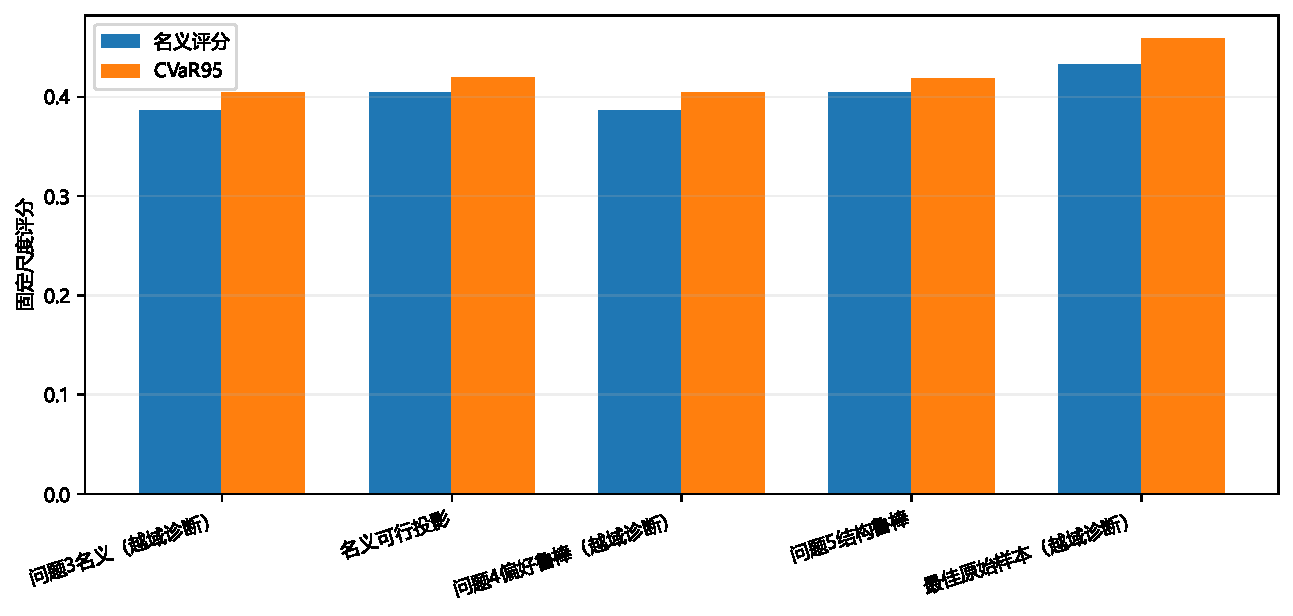
\includegraphics[width=.82\linewidth]{../figures/fig_q5_01_structure_risk.pdf}
\caption{域内候选的名义评分与加工尾部风险}
\end{figure}

独立均匀、对称三角、截断正态、正相关均匀、负相关均匀和确定性角点六种误差设定均选择同一$N=6$候选，CVaR95约位于0.4164至0.4208之间。这支持该方案对已声明误差模型的稳定性，但不代表真实制造分布已经由实验确定。

\section{工况扰动与模型不确定性}
以$s_m,s_q\in[0.95,1.05]$表示质量流量和热负荷尺度，构造弱、中、强三类流量敏感机制，并分别考虑两种温度非均匀性响应形式。六类情景用于压力测试，不替代真实变工况数据。各情景下专属最优的$N$可能为4或10，说明加工鲁棒不等于工况模型鲁棒。

对六类情景计算候选相对各情景专属最优的遗憾，最小最大模型遗憾候选为
\[
(a,b,N)=(0.231667,3.275,6),\qquad
\max r_{model}\approx0.179633.
\]
该方案适合作为工况模型不确定性较强时的保守备选，而不是现实工况全局最优。

\begin{figure}[H]\centering
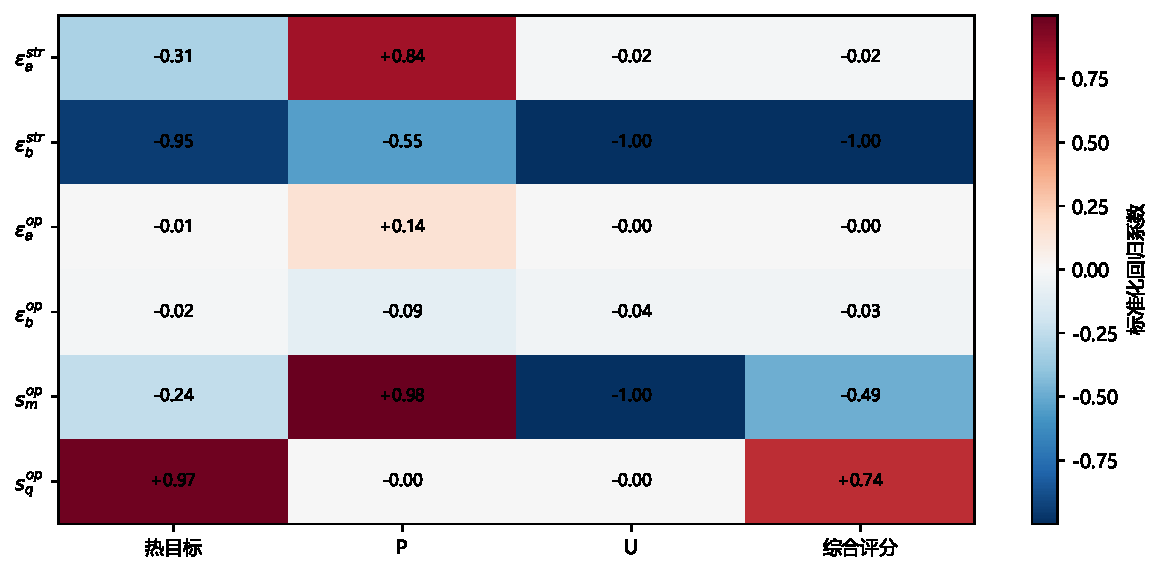
\includegraphics[width=.84\linewidth]{../figures/fig_q5_04_signed_sensitivity.pdf}
\caption{加工误差与代表工况下的带符号敏感性}
\end{figure}

全局敏感性显示，在代表工况中热负荷尺度$s_q$对综合风险的影响最大，其一阶Sobol指数约为0.711；质量流量尺度$s_m$约为0.240；几何加工偏差的全局贡献相对较小。综合评分的主导指标会在热阻、压降和温度非均匀性之间切换，因此单一线性敏感性系数不能完整代替全局分析。

\section{问题5结论}
在现有附件数据、给定加工误差范围和代理模型合法域内，采用$(0.224006,4.4625,6)$作为最终工程推荐。它兼顾名义性能、加工裕量和尾部风险。若未来获得真实变流量、变热负荷数据，应重新标定工况模型，再判断是否采用工况专用方案或跨模型保守方案。
\end{document}

